\frontmatter
\begin{titlepage}
\begin{tikzpicture}[remember picture,overlay]
\fill[fill={rgb,255:red,26;green,50;blue,99}] (current page.south west) rectangle (current page.north east);
\node[anchor=center] at ([yshift=-0.9in]current page.center) {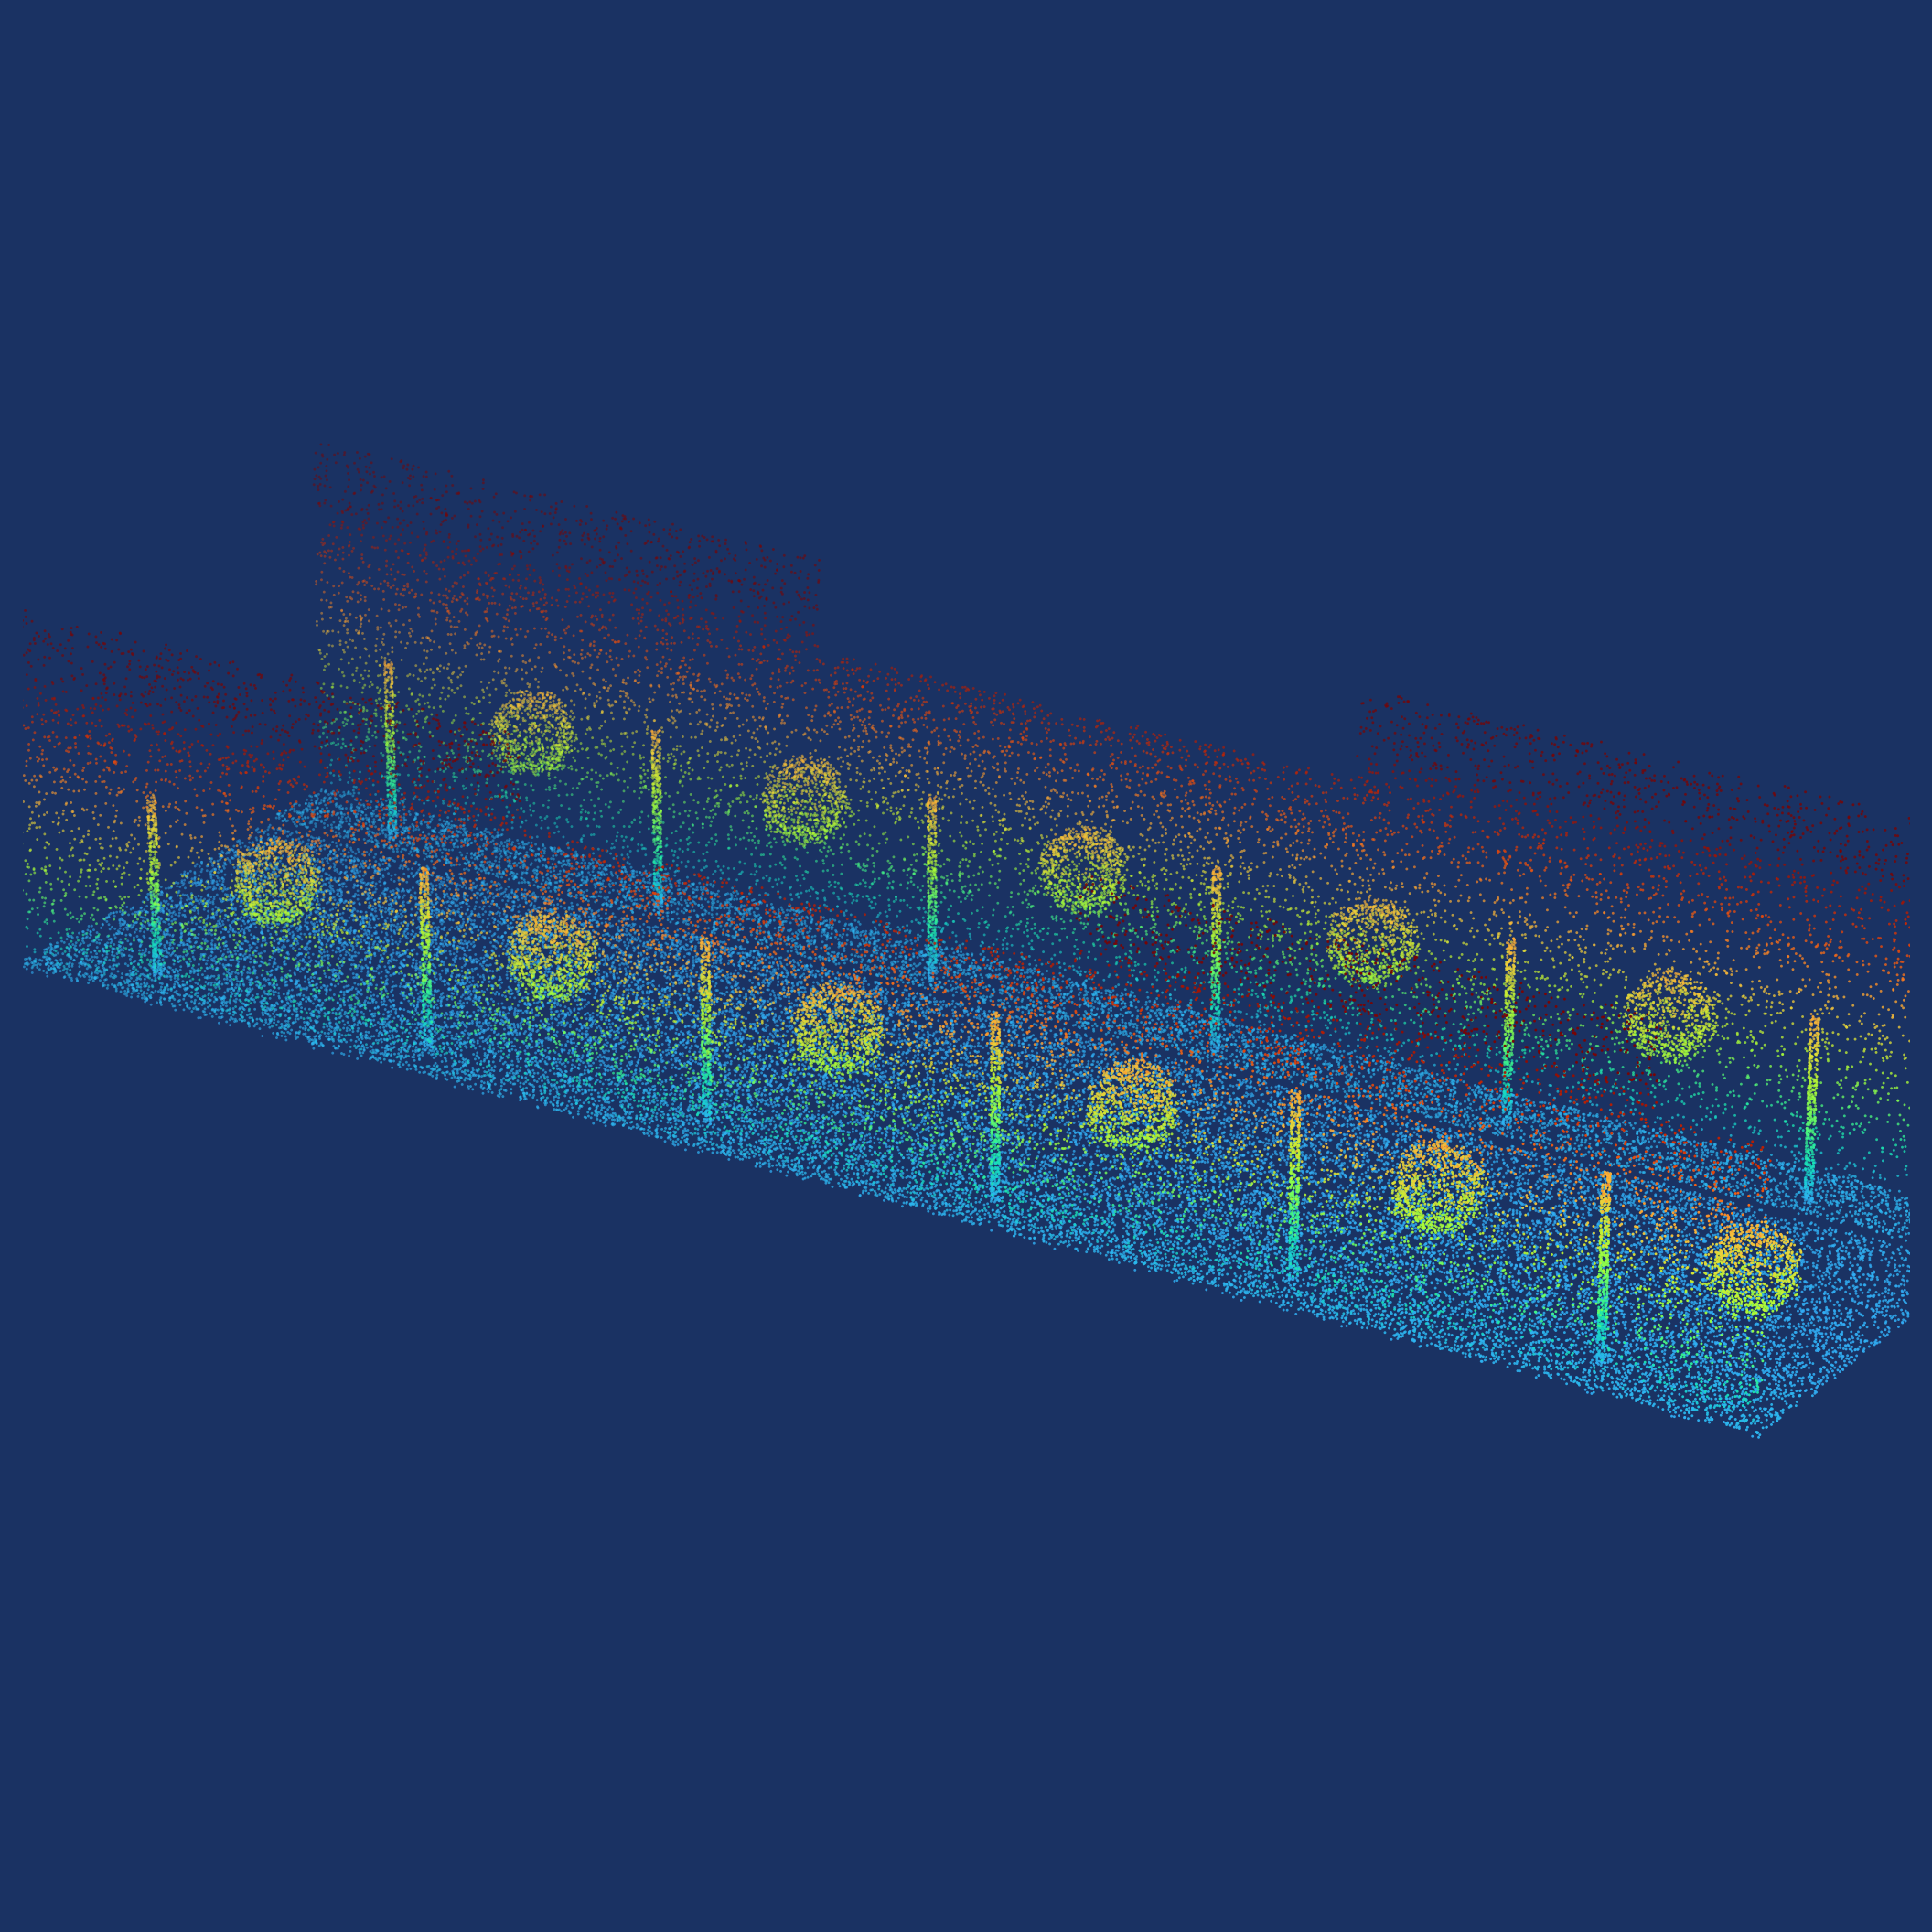
\includegraphics[width=\paperwidth]{cover}};
\fill[orange] ([yshift=-3.05in]current page.north west) rectangle ([yshift=-3.12in]current page.north east);
\node[anchor=north west,text width=7in,align=left] at ([xshift=0.75in,yshift=-0.8in]current page.north west)
 {\color{white}\sffamily\bfseries\fontsize{40}{46}\selectfont\spaceskip=0.28em LiDAR from the Ground Up};
\node[anchor=north west,text width=7in,align=left] at ([xshift=0.75in,yshift=-1.65in]current page.north west)
 {\color{orange!60}\sffamily\Large Surveying Concepts Edition};
\node[anchor=north west,text width=7in,align=left] at ([xshift=0.75in,yshift=-2.05in]current page.north west)
 {\color{white}\sffamily\bfseries\LARGE D.S. Banks, PSM};
\node[anchor=north west,text width=7in,align=left] at ([xshift=0.75in,yshift=-2.55in]current page.north west)
 {\color{white!85}\sffamily\large The core ideas of mobile LiDAR in plain language,\\ with field tips for surveyors.};
\node[anchor=south west,text width=7in,align=left] at ([xshift=0.75in,yshift=0.8in]current page.south west)
 {\color{white}\sffamily\large 21 modules \textbullet\ concepts, field tips and illustrations\\[6pt]
 \color{white!70}\sffamily\normalsize Course Text R1};
\end{tikzpicture}
\end{titlepage}

\chapter*{About This Edition}
\markboth{About This Edition}{}
This is the Surveying Concepts edition (R1) of \emph{LiDAR from the Ground Up}. It keeps the plain-language track of the full course: every green \textbf{Simple Approach} box, every \textbf{Big Idea}, every \textbf{Surveyor's Field Tip} and \textbf{Warning}, and the illustrations, in the same order and with the same module numbers as the full text.

The engineering track --- equations, worked examples, exercises, reference tables, labs, the sample SOP and the appendices --- is in the full course text (R0).

{\makeatletter\renewcommand*\l@chapter{\@dottedtocline{0}{0em}{1.8em}}\makeatother
\tableofcontents}
\clearpage\pagenumbering{arabic}\makeatletter\@mainmattertrue\@openrightfalse\makeatother
